%\SweaveUTF8
\documentclass[aspectratio=169]{beamer}

\usetheme{default}
% Slide setup, colour independent

\usepackage{amsmath,amssymb,amsthm}
\usepackage[utf8]{inputenc}
\usepackage{colortbl}
\usepackage{bm}
\usepackage{xcolor}
\usepackage{dsfont}
\usepackage{setspace}
%\usepackage{subfigure}
% To use \ding{234} and the like
\usepackage{pifont}
% To cross reference between slide files
\usepackage{zref-xr,zref-user}
% Use something like
% \zexternaldocument{fileI}
% in the tex files. And cite using \zref instead of \ref
\usepackage{booktabs}
\usepackage{marvosym}
\usepackage{cancel}
%\usepackage{transparent}

% Fields and the like
\def\IC{\mathbb{C}}
\def\IE{\mathbb{E}}
\def\IF{\mathbb{F}}
\def\II{\mathbb{I}}
\def\IJ{\mathbb{J}}
\def\IK{\mathbb{K}}
\def\IM{\mathbb{M}}
\def\IN{\mathbb{N}}
\def\IP{\mathbb{P}}
\def\IR{\mathbb{R}}
\def\IZ{\mathbb{Z}}
\def\11{\mathds{1}}


% Bold lowercase
\def\ba{\bm{a}}
\def\bb{\bm{b}}
\def\bc{\bm{c}}
\def\bd{\bm{d}}
\def\be{\bm{e}}
\def\bf{\bm{f}}
\def\bh{\bm{h}}
\def\bi{\bm{i}}
\def\bj{\bm{j}}
\def\bk{\bm{k}}
\def\bn{\bm{n}}
\def\bp{\bm{p}}
\def\br{\bm{r}}
\def\bs{\bm{s}}
\def\bu{\bm{u}}
\def\bv{\bm{v}}
\def\bw{\bm{w}}
\def\bx{\bm{x}}
\def\by{\bm{y}}
\def\bz{\bm{z}}

% Bold capitals
\def\bB{\bm{B}}
\def\bD{\bm{D}}
\def\bE{\bm{E}}
\def\bF{\bm{F}}
\def\bG{\bm{G}}
\def\bI{\bm{I}}
\def\bL{\bm{L}}
\def\bN{\bm{N}}
\def\bP{\bm{P}}
\def\bR{\bm{R}}
\def\bS{\bm{S}}
\def\bT{\bm{T}}
\def\bX{\bm{X}}

% Bold numbers
\def\b0{\bm{0}}

% Bold greek
\bmdefine{\bmu}{\bm{\mu}}
\def\bphi{\bm{\phi}}
\def\bvarphi{\bm{\varphi}}
\def\bPi{\bm{\Pi}}
\def\bGamma{\bm{\Gamma}}

% Bold red sentence
\def\boldred#1{{\color{red}\textbf{#1}}}
\def\defword#1{{\color{orange}\textbf{#1}}}

% Caligraphic letters
\def\A{\mathcal{A}}
\def\B{\mathcal{B}}
\def\C{\mathcal{C}}
\def\D{\mathcal{D}}
\def\E{\mathcal{E}}
\def\F{\mathcal{F}}
\def\G{\mathcal{G}}
\def\H{\mathcal{H}}
\def\I{\mathcal{I}}
\def\L{\mathcal{L}}
\def\M{\mathcal{M}}
\def\N{\mathcal{N}}
\def\P{\mathcal{P}}
\def\R{\mathcal{R}}
\def\S{\mathcal{S}}
\def\T{\mathcal{T}}
\def\U{\mathcal{U}}
\def\V{\mathcal{V}}

% Adding space for prime (') where needed
\def\pprime{\,'}
% Adding space for star (\star) where needed
\def\pstar{{\,\star}}

% tt font for code
\def\code#1{{\tt #1}}

% i.e., e.g.
\def\eg{\emph{e.g.}}
\def\ie{\emph{i.e.}}


% Operators and special symbols
\def\nbOne{{\mathchoice {\rm 1\mskip-4mu l} {\rm 1\mskip-4mu l}
{\rm 1\mskip-4.5mu l} {\rm 1\mskip-5mu l}}}
\def\cov{\ensuremath{\mathsf{cov}}}
\def\Var{\ensuremath{\mathsf{Var}\ }}
\def\Im{\textrm{Im}\;}
\def\Re{\textrm{Re}\;}
\def\det{\ensuremath{\mathsf{det}}}
\def\diag{\ensuremath{\mathsf{diag}}}
\def\nullspace{\ensuremath{\mathsf{null}}}
\def\nullity{\ensuremath{\mathsf{nullity}}}
\def\rank{\ensuremath{\mathsf{rank}}}
\def\range{\ensuremath{\mathsf{range}}}
\def\sgn{\ensuremath{\mathsf{sgn}}}
\def\Span{\ensuremath{\mathsf{span}}}
\def\tr{\ensuremath{\mathsf{tr}}}
\def\imply{$\Rightarrow$}
\def\restrictTo#1#2{\left.#1\right|_{#2}}
\newcommand{\parallelsum}{\mathbin{\!/\mkern-5mu/\!}}
\def\dsum{\mathop{\displaystyle \sum }}%
\def\dind#1#2{_{\substack{#1\\ #2}}}

\DeclareMathOperator{\GL}{GL}
\DeclareMathOperator{\Rel}{Re}
\def\Nt#1{\left|\!\left|\!\left|#1\right|\!\right|\!\right|}
\newcommand{\tripbar}{|\! |\! |}



% The beamer bullet (in base colour)
\def\bbullet{\leavevmode\usebeamertemplate{itemize item}\ }

% Theorems and the like
\newtheorem{proposition}[theorem]{Proposition}
\newtheorem{property}[theorem]{Property}
\newtheorem{importantproperty}[theorem]{Property}
\newtheorem{importanttheorem}[theorem]{Theorem}
%\newtheorem{lemma}[theorem]{Lemma}
%\newtheorem{corollary}[theorem]{Corollary}
\newtheorem{remark}[theorem]{Remark}
\setbeamertemplate{theorems}[numbered]
%\setbeamertemplate{theorems}[ams style]

%
%\usecolortheme{orchid}
%\usecolortheme{orchid}

\def\red{\color[rgb]{1,0,0}}
\def\blue{\color[rgb]{0,0,1}}
\def\green{\color[rgb]{0,1,0}}


% Get rid of navigation stuff
\setbeamertemplate{navigation symbols}{}

% Set footline/header line
\setbeamertemplate{footline}
{%
\quad p. \insertpagenumber \quad--\quad \insertsection\vskip2pt
}
% \setbeamertemplate{headline}
% {%
% \quad\insertsection\hfill p. \insertpagenumber\quad\mbox{}\vskip2pt
% }


\makeatletter
\newlength\beamerleftmargin
\setlength\beamerleftmargin{\Gm@lmargin}
\makeatother

% Colours for special pages
\def\extraContent{yellow!20}


%%%%%%%%%%%%%%%%%
\usepackage{tikz}
\usetikzlibrary{shapes,arrows}
\usetikzlibrary{positioning}
\usetikzlibrary{shapes.symbols,shapes.callouts,patterns}
\usetikzlibrary{calc,fit}
\usetikzlibrary{backgrounds}
\usetikzlibrary{decorations.pathmorphing,fit,petri}
\usetikzlibrary{automata}
\usetikzlibrary{fadings}
\usetikzlibrary{patterns,hobby}
\usetikzlibrary{backgrounds,fit,petri}
\usetikzlibrary{tikzmark}

\usepackage{pgfplots}
\pgfplotsset{compat=1.6}
\pgfplotsset{ticks=none}

\usetikzlibrary{decorations.markings}
\usetikzlibrary{arrows.meta}
\tikzset{>=stealth}

% For tikz
\tikzstyle{cloud} = [draw, ellipse,fill=red!20, node distance=0.87cm,
minimum height=2em]
\tikzstyle{line} = [draw, -latex']


%%% For max frame images
\newenvironment{changemargin}[2]{%
\begin{list}{}{%
\setlength{\topsep}{0pt}%
\setlength{\leftmargin}{#1}%
\setlength{\rightmargin}{#2}%
\setlength{\listparindent}{\parindent}%
\setlength{\itemindent}{\parindent}%
\setlength{\parsep}{\parskip}%
}%
\item[]}{\end{list}}


% Make one image take up the entire slide content area in beamer,.:
% centered/centred full-screen image, with title:
% This uses the whole screen except for the 1cm border around it
% all. 128x96mm
\newcommand{\titledFrameImage}[2]{
\begin{frame}{#1}
%\begin{changemargin}{-1cm}{-1cm}
\begin{center}
\includegraphics[width=108mm,height=\textheight,keepaspectratio]{#2}
\end{center}
%\end{changemargin}
\end{frame}
}

% Make one image take up the entire slide content area in beamer.:
% centered/centred full-screen image, no title:
% This uses the whole screen except for the 1cm border around it
% all. 128x96mm
\newcommand{\plainFrameImage}[1]{
\begin{frame}[plain]
%\begin{changemargin}{-1cm}{-1cm}
\begin{center}
\includegraphics[width=108mm,height=76mm,keepaspectratio]{#1}
\end{center}
%\end{changemargin}
\end{frame}
}

% Make one image take up the entire slide area, including borders, in beamer.:
% centered/centred full-screen image, no title:
% This uses the entire whole screen
\newcommand{\maxFrameImage}[1]{
\begin{frame}[plain]
\begin{changemargin}{-1cm}{-1cm}
\begin{center}
\includegraphics[width=\paperwidth,height=\paperheight,keepaspectratio]
{#1}
\end{center}
\end{changemargin}
\end{frame}
}

% This uses the entire whole screen (to include in frame)
\newcommand{\maxFrameImageNoFrame}[1]{
\begin{changemargin}{-1cm}{-1cm}
\begin{center}
\includegraphics[width=\paperwidth,height=0.99\paperheight,keepaspectratio]
{#1}
\end{center}
\end{changemargin}
}

% Make one image take up the entire slide area, including borders, in beamer.:
% centered/centred full-screen image, no title:
% This uses the entire whole screen
\newcommand{\maxFrameImageColor}[2]{
\begin{frame}[plain]
\setbeamercolor{normal text}{bg=#2!20}
\begin{changemargin}{-1cm}{-1cm}
\begin{center}
\includegraphics[width=\paperwidth,height=\paperheight,keepaspectratio]
{#1}
\end{center}
\end{changemargin}
\end{frame}
}


\usepackage{tikz}
\usetikzlibrary{patterns,hobby}
\usepackage{pgfplots}
\pgfplotsset{compat=1.6}
\pgfplotsset{ticks=none}

\usetikzlibrary{backgrounds}
\usetikzlibrary{decorations.markings}
\usetikzlibrary{arrows.meta}
\tikzset{>=stealth}

\tikzset{
  clockwise arrows/.style={
    postaction={
      decorate,
      decoration={
        markings,
        mark=between positions 0.1 and 0.9 step 40pt with {\arrow{>}},
   }}}}


% Beginning of a section
\newcommand{\newSectionSlide}[1]{
\begin{frame}[noframenumbering,plain]
  \begin{tikzpicture}[remember picture,overlay]
    \node[above right,inner sep=0pt,opacity=0.2] at (current page.south west)
    {
        \includegraphics[height=\paperheight,width=\paperwidth]{#1}
    };
  \end{tikzpicture}
  \setbeamercolor{section in toc}{fg=subsub_header_section}
  \setbeamerfont{section in toc}{size=\Large,series=\bfseries}
  \setbeamertemplate{section in toc shaded}[default][60]
  %\setbeamercolor{background canvas}{bg=section_colour}
  \tableofcontents[
    currentsection,
    sectionstyle=show/shaded,
    subsectionstyle=show/hide/hide,
    subsubsectionstyle=hide/hide/hide]
\end{frame}
\addtocounter{page}{-1}
}

% Beginning of a subsection
\newcommand{\newSubSectionSlide}[1]{
\begin{frame}[noframenumbering,plain]
  \begin{tikzpicture}[remember picture,overlay]
    \node[above right,inner sep=0pt,opacity=0.2] at (current page.south west)
    {
        \includegraphics[height=\paperheight,width=\paperwidth]{#1}
    };
  \end{tikzpicture}
  \setbeamercolor{section in toc}{fg=subsub_header_section}
  \setbeamerfont{section in toc}{size=\Large,series=\bfseries}
  \setbeamertemplate{section in toc shaded}[default][60]
  %\setbeamercolor{background canvas}{bg=section_colour}
  \tableofcontents[
    currentsection,
    sectionstyle=show/hide,
    subsectionstyle=show/shaded/hide,
    subsubsectionstyle=hide/hide/hide]
\end{frame}
\addtocounter{page}{-1}
}



   %%%%%%%%%%%
% To have links to parts in the outline
\makeatletter
\AtBeginPart{%
  \addtocontents{toc}{\protect\beamer@partintoc{\the\c@part}{\beamer@partnameshort}{\the\c@page}}%
}
%% number, shortname, page.
\providecommand\beamer@partintoc[3]{%
  \ifnum\c@tocdepth=-1\relax
    % requesting onlyparts.
    \makebox[6em]{Part #1:} \textcolor{green!30!blue}{\hyperlink{#2}{#2}}
    \par
  \fi
}
\define@key{beamertoc}{onlyparts}[]{%
  \c@tocdepth=-1\relax
}
\makeatother%

\newcommand{\nameofthepart}{}
\newcommand{\nupart}[1]%
    {   \part{#1}%
        \renewcommand{\nameofthepart}{#1}%
        {
          \setbeamercolor{background canvas}{bg=orange!50}
          \begin{frame}{#1}%\partpage 
          \hypertarget{\nameofthepart}{}\tableofcontents%
          \end{frame}
        }
    }


% The title page with figure
\newcommand{\titlepagewithfigure}[1]{%
\begin{frame}[noframenumbering,plain]
  \begin{tikzpicture}[remember picture,overlay]
    \node[above right,inner sep=0pt,opacity=0.2] at (current page.south west)
    {
        \includegraphics[height=\paperheight,width=\paperwidth]{#1}
    };
    \node[anchor=north east,
    inner sep=5pt,
    opacity=0.9] at (current page.north east)
    {
        
\includegraphics[width=0.2\textwidth]{FIGS/UM-logo-horizontal-CMYK.png}
    };
    \node[anchor=south, 
    align=justify, 
    text=black, 
    text width=1.1\textwidth,
    font=\footnotesize]  (land_acknowledgement)
    at (current page.south) 
    {The University of Manitoba campuses are located on original lands of Anishinaabeg, Ininew, Anisininew, Dakota and Dene peoples, and on the National Homeland of the Red River Métis.\\
    We respect the Treaties that were made on these territories, we acknowledge the harms and mistakes of the past, and we dedicate ourselves to move forward in partnership with Indigenous communities in a spirit of Reconciliation and collaboration.};  
    \node[align=center, anchor=south,
    above=0.5cm of land_acknowledgement,
    text=black,
    font=\bfseries] {Fall 2024};
\end{tikzpicture}
  \setbeamercolor{title}{fg=subsub_header_section}
  \setbeamercolor{author}{fg=subsub_header_section} 
  \setbeamerfont{title}{size=\Large,series=\bfseries}
  \setbeamerfont{author}{size=\Large,series=\bfseries}
  \setbeamerfont{date}{series=\bfseries}
	\titlepage
\end{frame}
\addtocounter{page}{-1}
}


% The outline page, with figure
\newcommand{\outlinepage}[1]{%
\begin{frame}[noframenumbering,plain]
  \begin{tikzpicture}[remember picture,overlay]
    \node[above right,inner sep=0pt,opacity=0.2] at (current page.south west)
    {
        \includegraphics[height=\paperheight,width=\paperwidth]{#1}
    };
  \end{tikzpicture}
  \setbeamercolor{section in toc}{fg=subsub_header_section}
  \setbeamerfont{section in toc}{size=\Large,series=\bfseries}
  \frametitle{\textcolor{blue}{\LARGE\bfseries Outline}}
  \tableofcontents[hideallsubsections]
\end{frame}
\addtocounter{page}{-1}
}




\usecolortheme{orchid}
%% Listings
\usepackage{listings}
\definecolor{mygreen}{rgb}{0,0.6,0}
\definecolor{mygray}{rgb}{0.5,0.5,0.5}
\definecolor{mymauve}{rgb}{0.58,0,0.82}
\definecolor{mygold}{rgb}{1,0.843,0}
\definecolor{myblue}{rgb}{0.537,0.812,0.941}

\definecolor{mygold2}{RGB}{120,105,22}
\definecolor{mygrey2}{RGB}{50,50,50}

\definecolor{lgreen}{rgb}{0.6,0.9,.6}
\definecolor{lred}{rgb}{1,0.5,.5}

\lstloadlanguages{R}
\lstset{ %
  language=R,
  backgroundcolor=\color{black!05},   % choose the background color
  basicstyle=\footnotesize\ttfamily,        % size of fonts used for the code
  breaklines=true,                 % automatic line breaking only at whitespace
  captionpos=b,                    % sets the caption-position to bottom
  commentstyle=\color{mygreen},    % comment style
  escapeinside={\%*}{*)},          % if you want to add LaTeX within your code
  keywordstyle=\color{red},       % keyword style
  stringstyle=\color{mygold},     % string literal style
  keepspaces=true,
  columns=fullflexible,
  tabsize=4,
}
% Could also do (in lstset)
% basicstyle==\fontfamily{pcr}\footnotesize
\lstdefinelanguage{Renhanced}%
  {keywords={abbreviate,abline,abs,acos,acosh,action,add1,add,%
      aggregate,alias,Alias,alist,all,anova,any,aov,aperm,append,apply,%
      approx,approxfun,apropos,Arg,args,array,arrows,as,asin,asinh,%
      atan,atan2,atanh,attach,attr,attributes,autoload,autoloader,ave,%
      axis,backsolve,barplot,basename,besselI,besselJ,besselK,besselY,%
      beta,binomial,body,box,boxplot,break,browser,bug,builtins,bxp,by,%
      c,C,call,Call,case,cat,category,cbind,ceiling,character,char,%
      charmatch,check,chol,chol2inv,choose,chull,class,close,cm,codes,%
      coef,coefficients,co,col,colnames,colors,colours,commandArgs,%
      comment,complete,complex,conflicts,Conj,contents,contour,%
      contrasts,contr,control,helmert,contrib,convolve,cooks,coords,%
      distance,coplot,cor,cos,cosh,count,fields,cov,covratio,wt,CRAN,%
      create,crossprod,cummax,cummin,cumprod,cumsum,curve,cut,cycle,D,%
      data,dataentry,date,dbeta,dbinom,dcauchy,dchisq,de,debug,%
      debugger,Defunct,default,delay,delete,deltat,demo,de,density,%
      deparse,dependencies,Deprecated,deriv,description,detach,%
      dev2bitmap,dev,cur,deviance,off,prev,,dexp,df,dfbetas,dffits,%
      dgamma,dgeom,dget,dhyper,diag,diff,digamma,dim,dimnames,dir,%
      dirname,dlnorm,dlogis,dnbinom,dnchisq,dnorm,do,dotplot,double,%
      download,dpois,dput,drop,drop1,dsignrank,dt,dummy,dump,dunif,%
      duplicated,dweibull,dwilcox,dyn,edit,eff,effects,eigen,else,%
      emacs,end,environment,env,erase,eval,equal,evalq,example,exists,%
      exit,exp,expand,expression,External,extract,extractAIC,factor,%
      fail,family,fft,file,filled,find,fitted,fivenum,fix,floor,for,%
      For,formals,format,formatC,formula,Fortran,forwardsolve,frame,%
      frequency,ftable,ftable2table,function,gamma,Gamma,gammaCody,%
      gaussian,gc,gcinfo,gctorture,get,getenv,geterrmessage,getOption,%
      getwd,gl,glm,globalenv,gnome,GNOME,graphics,gray,grep,grey,grid,%
      gsub,hasTsp,hat,heat,help,hist,home,hsv,httpclient,I,identify,if,%
      ifelse,Im,image,\%in\%,index,influence,measures,inherits,install,%
      installed,integer,interaction,interactive,Internal,intersect,%
      inverse,invisible,IQR,is,jitter,kappa,kronecker,labels,lapply,%
      layout,lbeta,lchoose,lcm,legend,length,levels,lgamma,library,%
      licence,license,lines,list,lm,load,local,locator,log,log10,log1p,%
      log2,logical,loglin,lower,lowess,ls,lsfit,lsf,ls,machine,Machine,%
      mad,mahalanobis,make,link,margin,match,Math,matlines,mat,matplot,%
      matpoints,matrix,max,mean,median,memory,menu,merge,methods,min,%
      missing,Mod,mode,model,response,mosaicplot,mtext,mvfft,na,nan,%
      names,omit,nargs,nchar,ncol,NCOL,new,next,NextMethod,nextn,%
      nlevels,nlm,noquote,NotYetImplemented,NotYetUsed,nrow,NROW,null,%
      numeric,\%o\%,objects,offset,old,on,Ops,optim,optimise,optimize,%
      options,or,order,ordered,outer,package,packages,page,pairlist,%
      pairs,palette,panel,par,parent,parse,paste,path,pbeta,pbinom,%
      pcauchy,pchisq,pentagamma,persp,pexp,pf,pgamma,pgeom,phyper,pico,%
      pictex,piechart,Platform,plnorm,plogis,plot,pmatch,pmax,pmin,%
      pnbinom,pnchisq,pnorm,points,poisson,poly,polygon,polyroot,pos,%
      postscript,power,ppoints,ppois,predict,preplot,pretty,Primitive,%
      print,prmatrix,proc,prod,profile,proj,prompt,prop,provide,%
      psignrank,ps,pt,ptukey,punif,pweibull,pwilcox,q,qbeta,qbinom,%
      qcauchy,qchisq,qexp,qf,qgamma,qgeom,qhyper,qlnorm,qlogis,qnbinom,%
      qnchisq,qnorm,qpois,qqline,qqnorm,qqplot,qr,Q,qty,qy,qsignrank,%
      qt,qtukey,quantile,quasi,quit,qunif,quote,qweibull,qwilcox,%
      rainbow,range,rank,rbeta,rbind,rbinom,rcauchy,rchisq,Re,read,csv,%
      csv2,fwf,readline,socket,real,Recall,rect,reformulate,regexpr,%
      relevel,remove,rep,repeat,replace,replications,report,require,%
      resid,residuals,restart,return,rev,rexp,rf,rgamma,rgb,rgeom,R,%
      rhyper,rle,rlnorm,rlogis,rm,rnbinom,RNGkind,rnorm,round,row,%
      rownames,rowsum,rpois,rsignrank,rstandard,rstudent,rt,rug,runif,%
      rweibull,rwilcox,sample,sapply,save,scale,scan,scan,screen,sd,se,%
      search,searchpaths,segments,seq,sequence,setdiff,setequal,set,%
      setwd,show,sign,signif,sin,single,sinh,sink,solve,sort,source,%
      spline,splinefun,split,sqrt,stars,start,stat,stem,step,stop,%
      storage,strstrheight,stripplot,strsplit,structure,strwidth,sub,%
      subset,substitute,substr,substring,sum,summary,sunflowerplot,svd,%
      sweep,switch,symbol,symbols,symnum,sys,status,system,t,table,%
      tabulate,tan,tanh,tapply,tempfile,terms,terrain,tetragamma,text,%
      time,title,topo,trace,traceback,transform,tri,trigamma,trunc,try,%
      ts,tsp,typeof,unclass,undebug,undoc,union,unique,uniroot,unix,%
      unlink,unlist,unname,untrace,update,upper,url,UseMethod,var,%
      variable,vector,Version,vi,warning,warnings,weighted,weights,%
      which,while,window,write,\%x\%,x11,X11,xedit,xemacs,xinch,xor,%
      xpdrows,xy,xyinch,yinch,zapsmall,zip},%
   otherkeywords={!,!=,~,$,*,\%,\&,\%/\%,\%*\%,\%\%,<-,<<-,_,/},%
   alsoother={._$},%
   sensitive,%
   morecomment=[l]\#,%
   morestring=[d]",%
   morestring=[d]'% 2001 Robert Denham
  }%

%%%%%%% 
%% Definitions in yellow boxes
\usepackage{etoolbox}
\setbeamercolor{block title}{use=structure,fg=structure.fg,bg=structure.fg!40!bg}
\setbeamercolor{block body}{parent=normal text,use=block title,bg=block title.bg!20!bg}

\BeforeBeginEnvironment{definition}{%
	\setbeamercolor{block title}{fg=black,bg=yellow!20!white}
	\setbeamercolor{block body}{fg=black, bg=yellow!05!white}
}
\AfterEndEnvironment{definition}{
	\setbeamercolor{block title}{use=structure,fg=structure.fg,bg=structure.fg!20!bg}
	\setbeamercolor{block body}{parent=normal text,use=block title,bg=block title.bg!50!bg, fg=black}
}
\BeforeBeginEnvironment{importanttheorem}{%
	\setbeamercolor{block title}{fg=black,bg=red!20!white}
	\setbeamercolor{block body}{fg=black, bg=red!05!white}
}
\AfterEndEnvironment{importanttheorem}{
	\setbeamercolor{block title}{use=structure,fg=structure.fg,bg=structure.fg!20!bg}
	\setbeamercolor{block body}{parent=normal text,use=block title,bg=block title.bg!50!bg, fg=black}
}
\BeforeBeginEnvironment{importantproperty}{%
	\setbeamercolor{block title}{fg=black,bg=red!50!white}
	\setbeamercolor{block body}{fg=black, bg=red!30!white}
}
\AfterEndEnvironment{importantproperty}{
	\setbeamercolor{block title}{use=structure,fg=structure.fg,bg=structure.fg!20!bg}
	\setbeamercolor{block body}{parent=normal text,use=block title,bg=block title.bg!50!bg, fg=black}
}

% Colour for the outline page
\definecolor{outline_colour}{RGB}{230,165,83}
%% Colours for sections, subsections aand subsubsections
\definecolor{section_colour}{RGB}{27,46,28}
\definecolor{subsection_colour}{RGB}{52,128,56}
\definecolor{subsubsection_colour}{RGB}{150,224,154}
\definecolor{subsub_header_section}{RGB}{196,44,27}
%\definecolor{mygold}{rgb}{1,0.843,0}
% Beginning of a section
% \AtBeginSection[]{
% 	{
% 	  \setbeamercolor{section in toc}{fg=mygold}
% 		\setbeamercolor{background canvas}{bg=section_colour}
% 		\begin{frame}[noframenumbering,plain]
% 			\framesubtitle{\nameofthepart Chapter \insertromanpartnumber \ -- \iteminsert{\insertpart}}
% 			\tableofcontents[
% 				currentsection,
% 				sectionstyle=show/shaded,
% 				subsectionstyle=show/hide/hide,
% 				subsubsectionstyle=hide/hide/hide]
% 		\end{frame}
% 	\addtocounter{page}{-1}
% 	%\addtocounter{framenumber}{-1} 
% 	}
% }


% % Beginning of a section
% \AtBeginSubsection[]{
% 	{
% 	  \setbeamercolor{section in toc}{fg=mygold}
% 		\setbeamercolor{background canvas}{bg=subsection_colour}
% 		\begin{frame}[noframenumbering,plain]
% 				\framesubtitle{\nameofthepart Chapter \insertromanpartnumber \ -- \iteminsert{\insertpart}}
% 				\tableofcontents[
% 					currentsection,
% 					sectionstyle=show/hide,
% 					currentsubsection,
% 					subsectionstyle=show/shaded/hide,
% 					subsubsectionstyle=show/hide/hide]
% 			\end{frame}
% 		\addtocounter{page}{-1}
% 	}
% }

% \newcommand{\newSubSectionSlide}[1]{
% \begin{frame}[noframenumbering,plain]
%   \begin{tikzpicture}[remember picture,overlay]
%     \node[above right,inner sep=0pt,opacity=0.2] at (current page.south west)
%     {
%         \includegraphics[height=\paperheight,width=\paperwidth]{#1}
%     };
%   \end{tikzpicture}
%   \setbeamercolor{section in toc}{fg=subsub_header_section}
%   \setbeamerfont{section in toc}{size=\Large,series=\bfseries}
%   \setbeamertemplate{section in toc shaded}[default][60]
%   \setbeamertemplate{subsection in toc shaded}[default][60]
%   %\setbeamercolor{background canvas}{bg=section_colour}
%   \tableofcontents[
%     currentsection,
%     sectionstyle=show/hide,
%     currentsubsection,
%     subsectionstyle=show/shaded/hide,
%     subsubsectionstyle=show/hide/hide]
% \end{frame}
% \addtocounter{page}{-1}
% }


% Beginning of a section
\AtBeginSubsubsection[]{
	{
	  \setbeamercolor{section in toc}{fg=subsub_header_section}
	  \setbeamercolor{subsubsection in toc}{fg=mygold2}
	  \setbeamercolor{subsubsection in toc shaded}{fg=mygrey2}
		\setbeamercolor{background canvas}{bg=subsubsection_colour}
		\begin{frame}[noframenumbering,plain]
				\framesubtitle{\nameofthepart Chapter \insertromanpartnumber \ -- \iteminsert{\insertpart}}
				\tableofcontents[
					currentsection,
					sectionstyle=show/hide,
					currentsubsection,
					subsectionstyle=show/hide/shaded
					currentsubsubsection]%,
					%subsubsectionstyle=hide/hide/shaded]
					%currentsubsubsection]
			\end{frame}
		\addtocounter{page}{-1}
	}
}


\title[Identification of parameters]{Identification of parameters\\ Regression and Numerical integration}
\author{\texorpdfstring{Julien Arino\newline University of Manitoba\newline\url{julien.arino@umanitoba.ca}}{Julien Arino}}
\date{}


%%%%%%%%%%%%%%%%
\usepackage{Sweave}
\begin{document}
\input{math-3610-09-parameter-identification-concordance}




%%%%%%%%%%%%%%%%%%%%%%%%%%%%%%%%%
%%%%%%%%%%%%%%%%%%%%%%%%%%%%%%%%%
%%%%%%%%%%%%%%%%%%%%%%%%%%%%%%%%%
%%%%%%%%%%%%%%%%%%%%%%%%%%%%%%%%%
% The title page
\begin{frame}[noframenumbering,plain]
  \begin{tikzpicture}[remember picture,overlay]
    \node[above right,inner sep=0pt,opacity=0.2] at (current page.south west)
    {
        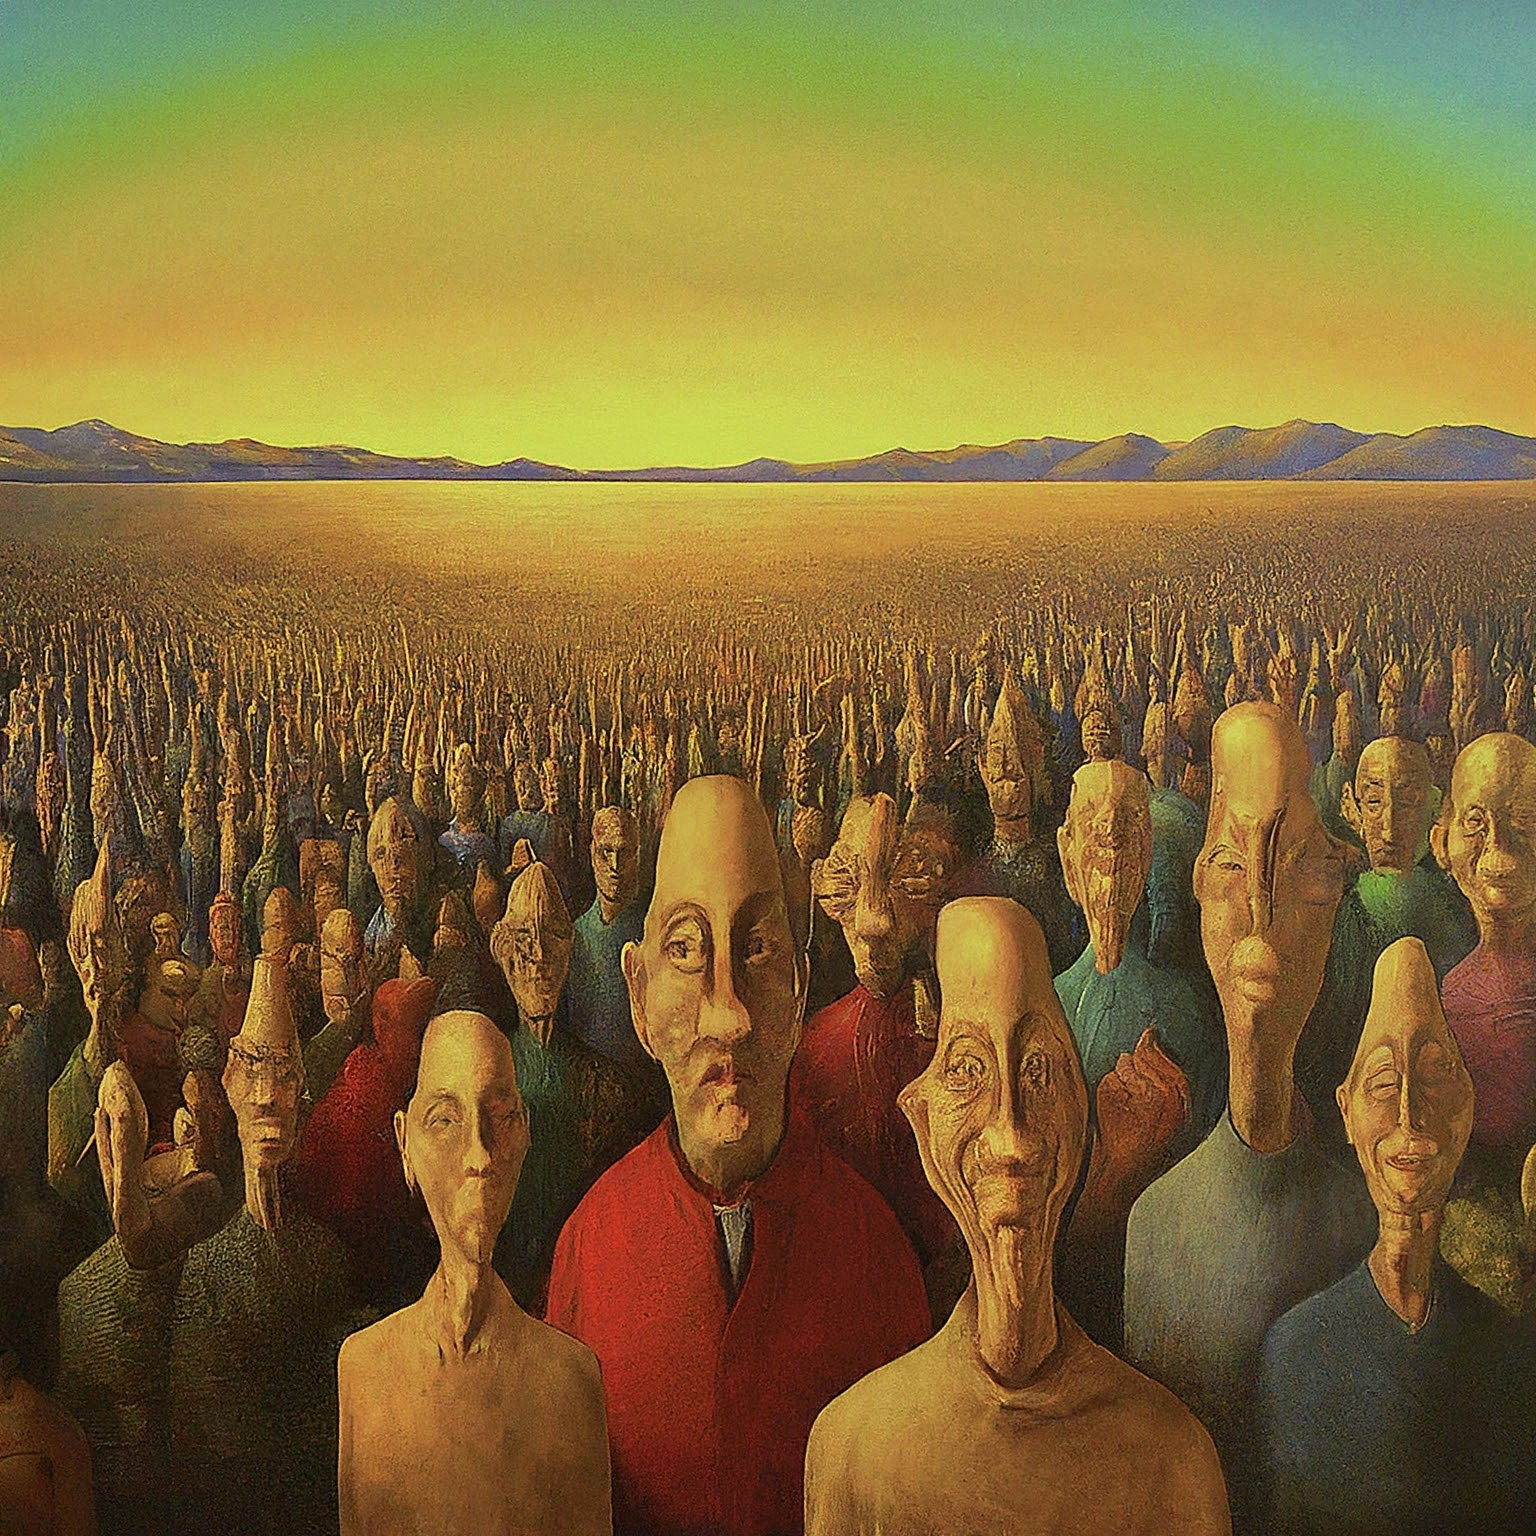
\includegraphics[height=\paperheight,width=\paperwidth]{FIGS/population-models-Gemini_Generated_Image_r55bcer55bcer55b.jpeg}
    };
    \node[anchor=north east,
    inner sep=5pt,
    opacity=0.9] at (current page.north east)
    {
        
\includegraphics[width=0.2\textwidth]{FIGS/UM-logo-horizontal-CMYK.png}
    };
    \node[anchor=south, 
    align=justify, 
    text=black, 
    text width=1.1\textwidth,
    font=\footnotesize]  (land_acknowledgement)
    at (current page.south) 
    {The University of Manitoba campuses are located on original lands of Anishinaabeg, Ininew, Anisininew, Dakota and Dene peoples, and on the National Homeland of the Red River Métis.\\
    We respect the Treaties that were made on these territories, we acknowledge the harms and mistakes of the past, and we dedicate ourselves to move forward in partnership with Indigenous communities in a spirit of Reconciliation and collaboration.};  
    \node[align=center, anchor=south,
    above=0.5cm of land_acknowledgement,
    text=black,
    font=\bfseries] {Fall 2024};
\end{tikzpicture}
  \setbeamercolor{title}{fg=subsub_header_section}
  \setbeamercolor{author}{fg=subsub_header_section} 
  \setbeamerfont{title}{size=\Large,series=\bfseries}
  \setbeamerfont{author}{size=\Large,series=\bfseries}
  \setbeamerfont{date}{series=\bfseries}
	\titlepage
\end{frame}
\addtocounter{page}{-1}


%%%%%%%%%%%%%%%%%%%%%%%%%%%%%%%%%
%%%%%%%%%%%%%%%%%%%%%%%%%%%%%%%%%
%%%%%%%%%%%%%%%%%%%%%%%%%%%%%%%%%
%%%%%%%%%%%%%%%%%%%%%%%%%%%%%%%%%
% The outline page
\begin{frame}[noframenumbering,plain]
  \begin{tikzpicture}[remember picture,overlay]
    \node[above right,inner sep=0pt,opacity=0.2] at (current page.south west)
    {
        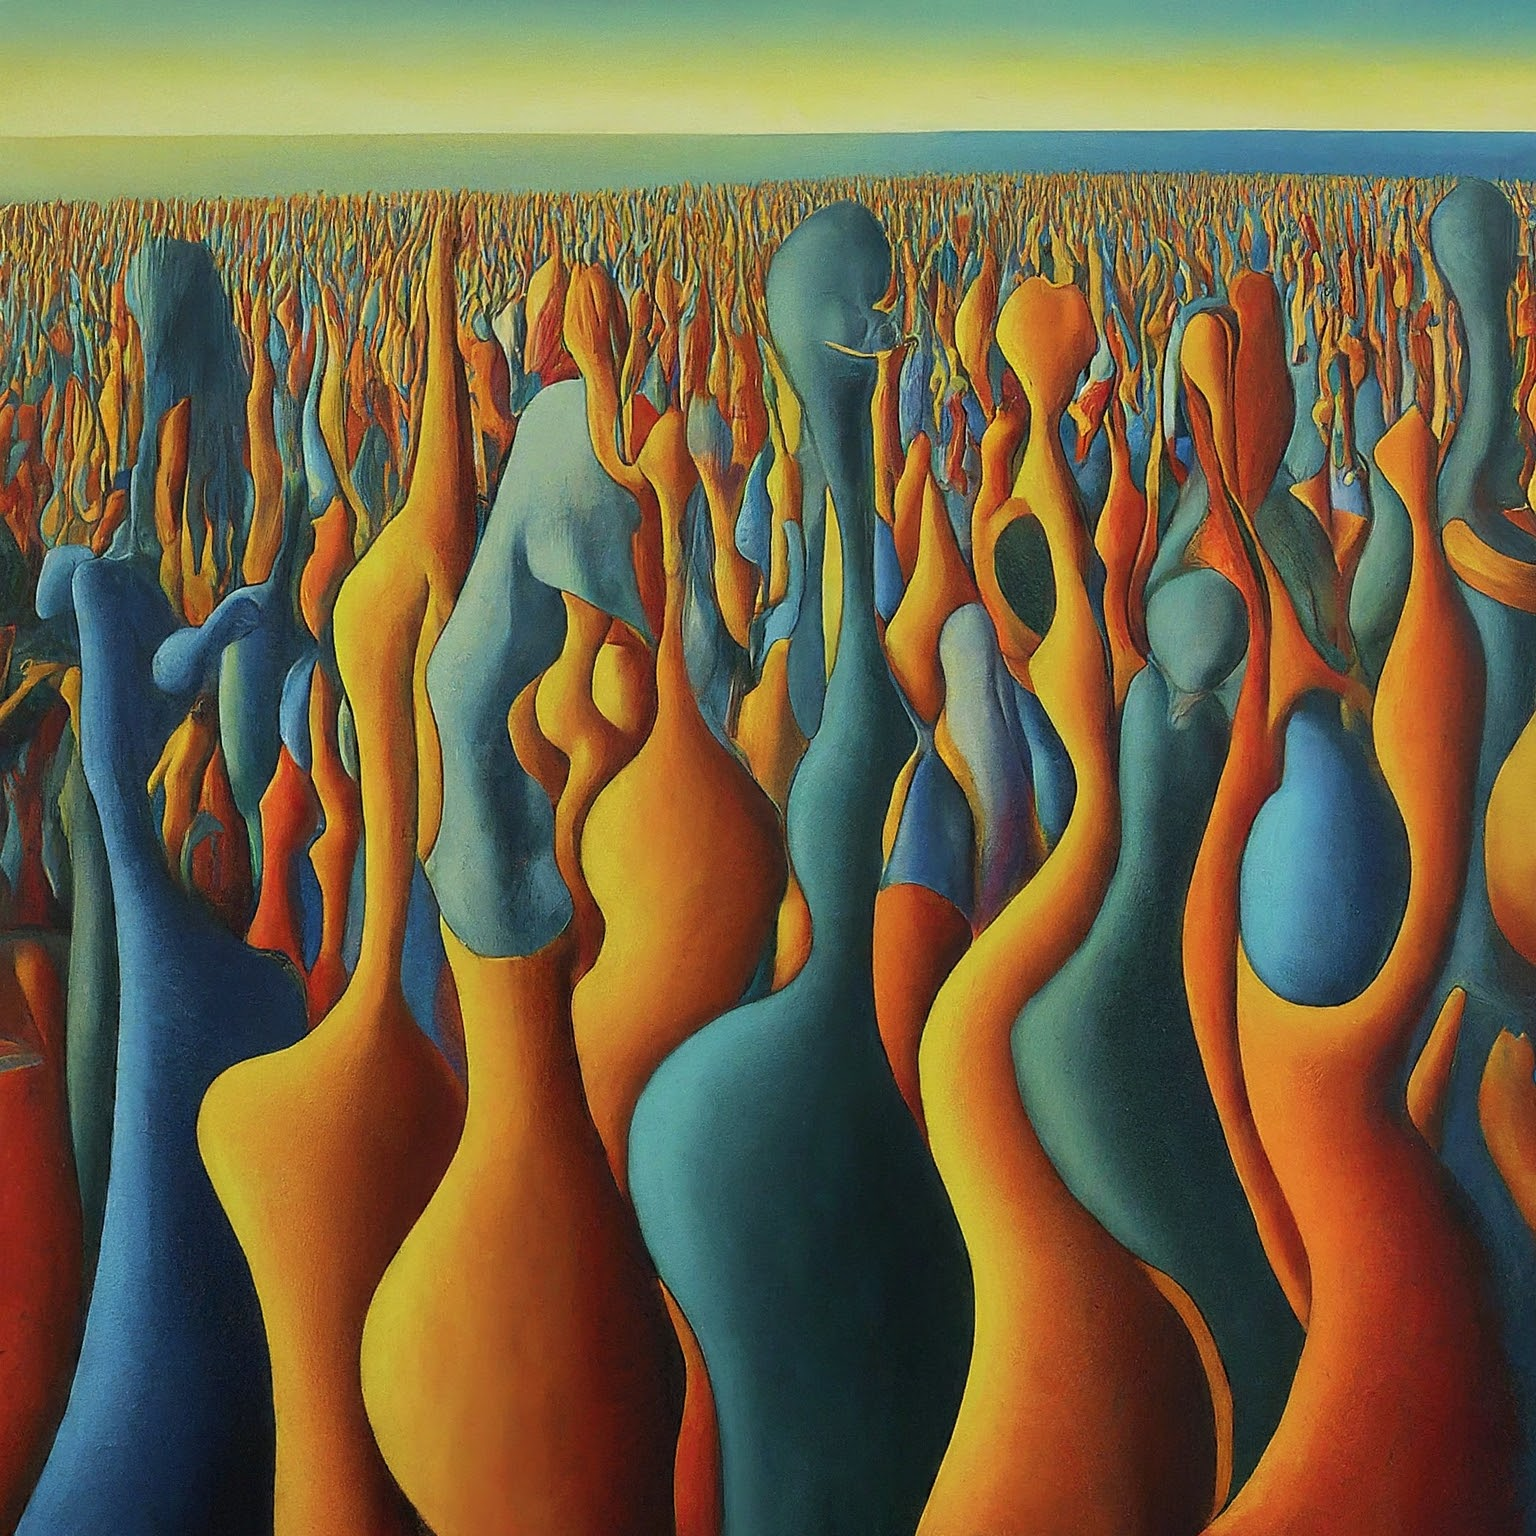
\includegraphics[height=\paperheight,width=\paperwidth]{FIGS/population-models-Gemini_Generated_Image_r55bccr55bccr55b.jpeg}
    };
  \end{tikzpicture}
  \setbeamercolor{section in toc}{fg=subsub_header_section}
  \setbeamerfont{section in toc}{size=\Large,series=\bfseries}
  \frametitle{\textcolor{blue}{\LARGE\bfseries Outline}}
  \tableofcontents[hideallsubsections]
\end{frame}
\addtocounter{page}{-1}



%%%%%%%%%%%%%%%%%%%
%%%%%%%%%%%%%%%%%%%
%%%%%%%%%%%%%%%%%%%
%%%%%%%%%%%%%%%%%%%
\section{Statement of the problem}
\frame[plain]{\tableofcontents[current]}

\frame{\frametitle{Objective}
We are given a table with the population census at different time intervals between a date $a$ and a date $b$, and we have a model to describe the evolution of this population
\vskip1cm
We want to \textbf{find parameters} of the model so that solutions of the model \textbf{fit} the data as well as possible 
}

\frame{\frametitle{Sources of uncertainty}
\begin{itemize}
\item Some parameters are known with reasonable accuracy. Others are known within a range of possible values
\item Data is obtained through measurement, and this measurement is not necessarily very precise
\item Data is usually intrinsically ``noisy''
\item The model you have is usually wrong (\textbf{all} models are wrong, the problem is to find one that is not too wrong, i.e., capable of answering your question)
\end{itemize}
Be aware of these limitations
}

\section{Case of the logistic equation}

\frame{\frametitle{The US population from 1790 to 2000 (revised numbers)}
\begin{center}
\begin{tabular}[t]{ccc}
\begin{tabular}{cc}
Year & Population\\
& (millions) \\
\hline
1790 & 3.929 \\
1800 & 5.308 \\
1810 & 7.240 \\
1820 & 9.638 \\
1830 & 12.866 \\
1840 & 17.069 \\
1850 & 23.192 \\
1860 & 31.443 \\
1870 & 38.558 \\
1880 & 50.156 \\
1890 & 62.948
\end{tabular} 
&\quad &
\begin{tabular}{cc}
Year & Population \\
& (millions) \\
\hline
1900 & 76.212 \\
1910 & 92.228 \\
1920 & 106.021 \\
1930 & 123.202 \\
1940 & 132.164 \\
1950 & 151.325 \\
1960 & 179.323 \\
1970 & 203.302 \\
1980 & 226.542 \\
1990 & 248.709 \\
2000 & 281.421
\end{tabular}
\end{tabular}
\end{center}
}

\frame{\frametitle{The logistic equation}
$r$ the intrinsic growth rate of the population, $K$ the carrying capacity,
\begin{equation}\label{eq:ode_logistic_ident}
N'=rN\left(1-\frac NK\right)\tag{Logistic}
\end{equation}
}

\frame{\frametitle{Parameter identification}
To identify parameters, we can use \textbf{nonlinear regression}. With the logistic equation, there are two methods:
\begin{enumerate}
\item Since the solution $N(t)$ to \eqref{eq:ode_logistic_ident} is known, we can use nonlinear regression directly on $N(t)$
\item We use nonlinear regression on the constructed (simulated) solution to \eqref{eq:ode_logistic_ident}
\end{enumerate}
}

\section{Using nonlinear regression}

\frame[containsverbatim]{\frametitle{Finding the solution of \eqref{eq:ode_logistic_ident} using maple}
\begin{verbatim}
eq := diff(N(t),t) = r*N(t)*(1-N(t)/K)
\end{verbatim}
\[
\frac{d}{dt}N(t)=rN(t)\left(1-\frac{N(t)}{K}\right)
\]
Solve without specifying an initial condition:
\begin{verbatim}
dsolve(eq, N(t))
\end{verbatim}
\[
N(t)=\frac{K}{1+e^{-rt}\_C1 K}
\]
Solve with initial condition $N(0)=C$:
\begin{verbatim}
dsolve({eq, N(t0) = C}, N(t))
\end{verbatim}
\[
N(t)=\frac{CKe^{-rt_0}}{Ce^{-rt_0}+e^{-rt}K-e^{-rt}C}
\]
}


\frame{
We use the solution
\[
N(t)=\frac{N_0Ke^{-rt_0}}{N_0e^{-rt_0}+e^{-rt}(K-N_0)}
\]
(we have replaced $C$ by $N_0$)
\vskip1cm
To reduce the number of parameters to find, we assume that the initial point is $(t_0,N_0)=(1790,3.929)$, the first data point
\vskip1cm
Note that we are working in millions (this is important later)
}


\frame{
Write the points as $(t_k,N_k)$, $k=2,\ldots,22$ --there are 22 data points, but we use the first as $(t_0,N_0)$ or, to make things more convenient to write, $(t_1,N_1)$. We want to minimize
\[
S=\sum_{k=2}^{22} \left(N(t_k)-N_k\right)^2,
\]
where $t_k$ are the known dates, $N_k$ are the known populations, and \[
N(t_k)=\frac{N_0Ke^{-rt_0}}{N_0e^{-rt_0}+e^{-rt_k}(K-N_0)}
\]
}

\frame{
Emphasize dependence on $r,K$:
\[
S(r,K)=\sum_{k=2}^{22} \left(
\frac{N_0Ke^{-rt_0}}{N_0e^{-rt_0}+e^{-rt_k}(K-N_0)}-N_k
\right)^2
\]
This is maximal if (necessary condition) $\partial S/\partial r=\partial S/\partial K=0$. 
}

\frame{
We have, for a given $k=2,\ldots,22$,
\begin{multline*}
\frac 12\;\frac{\partial}{\partial r}
\left(
\frac{N_0Ke^{-rt_0}}{N_0e^{-rt_0}+e^{-rt_k}(K-N_0)}-N_k
\right)^2 = \\
\frac
{K \left( N_k (N_0-K) e^{-rt_k}+
N_0e^{-rt_0}(K-N_k)  \right) 
N_0e^{-r(t_0+t_k)}(t_0-t_k)(N_0-K) }
{ \left( N_0{e^{-rt_0}}+{e^{-rt_k}}(K-N_0)  \right) ^3}
\end{multline*}
and
\begin{multline*}
\frac 12\;\frac{\partial}{\partial K}
\left(
\frac{N_0Ke^{-rt_0}}{N_0e^{-rt_0}+e^{-rt_k}(K-N_0)}-N_k
\right)^2 = \\
\frac 
{\left(e^{-rt_0}-e^{-rt_k}\right)  
\left(N_k(N_0-K)e^{-rt_k}+N_0e^{-rt_0}
(K-N_k)  \right) {N_0}^2{e^{-rt_0}}}
{\left(N_0e^{-rt_0}+e^{-rt_k}(K-N_0)\right)^3}
\end{multline*}
}

\frame{
So $\partial S/\partial r=0\Leftrightarrow$
\[
\left(N_k (N_0-K) e^{-rt_k}+N_0e^{-rt_0}(K-N_k)\right) 
N_0e^{-r(t_0+t_k)}(t_0-t_k)(N_0-K)=0
\]
(provided $\left(N_0{e^{-rt_0}}+{e^{-rt_k}}(K-N_0)\right) ^3\neq 0$)
\vskip0.5cm 
That is $\partial S/\partial r=0\Leftrightarrow$
\begin{equation}\label{eq:constraint1_regression}
N_k (N_0-K) e^{-rt_k}+N_0e^{-rt_0}(K-N_k)=0 \tag{*}
\end{equation}
or
\[
t_0-t_k=0\qquad\textrm{or}\qquad N_0-K=0
\]
The case $t_0=t_k$ cannot happen, since $k=2,\ldots,22$ (and we assume we do not have two different measurements for one time value). So we have either $K=N_0$ or \eqref{eq:constraint1_regression}
}

\frame{
Solving \eqref{eq:constraint1_regression} for $r$, we get
\[
r=-\frac{\ln\left(\frac{N_0(K-N_k)}{N_k(K-N_0)}\right)}{t_k-t_0}
=\frac{\ln\left(\frac{N_k(K-N_0)}{N_0(K-N_k)}\right)}{t_k-t_0}
\]
}

\frame{
Also $\partial S/\partial K=0\Leftrightarrow$
\[
\left(e^{-rt_0}-e^{-rt_k}\right)  
\left(N_k(N_0-K)e^{-rt_k}+N_0e^{-rt_0}
(K-N_k)  \right)=0
\]
(provided $\left(N_0e^{-rt_0}+e^{-rt_k}(K-N_0)\right)^3\neq 0$)
\vskip0.5cm
That is, $\partial S/\partial K=0\Leftrightarrow$
\[
e^{-rt_0}-e^{-rt_k}=0
\]
or
\begin{equation}\label{eq:constraint2_regression}
N_k(N_0-K)e^{-rt_k}+N_0e^{-rt_0}(K-N_k)=0\tag{**}
\end{equation}
The first condition implies $t_0=t_k$, which is impossible. So we are left with \eqref{eq:constraint2_regression}, which is the same equation as \eqref{eq:constraint1_regression}
}

\frame{
So this is a difficult problem.. (see the theory for nonlinear least squares if you are interested)
\vskip1cm
So we use plan B: numerics directly..
}


\section{Using simulations}

\frame{\frametitle{What we need to do}
Let us forget that we know the explicit solution to \eqref{eq:ode_logistic_ident}
\vskip0.5cm
\begin{itemize}
\item The solution to \eqref{eq:ode_logistic_ident} can be approximated numerically
\item We can construct one such numerical solution for given values of $r$ and $K$
\item We then can see ``how far off'' that solution is from our data points
\item We change the parameters $r$ and $K$ a little, find out ``how far off'' the new solution is from the data points
\item And repeat until we have found a solution that is better than others..
\end{itemize}
}


\frame{\frametitle{Finding the numerical solution to \eqref{eq:ode_logistic_ident}}
We can use
\begin{itemize}
\item matlab
\item octave
\item scilab
\item maple
\item mathematica
\item many others..
\end{itemize}
matlab, octave and scilab are recommended because of the ``philosophy''
}


\frame{\frametitle{Using matlab}
In matlab (and octave) the philosophy is very close to the ``natural'' way one proceeds with an ode: given the ODE
\[
x'=f(t,x)
\]
we must define the right hand side (RHS) function (the vector field) $f(t,x)$, and use it to compute the (numerical) solution
}

\frame{\frametitle{Reminder: Euler's method}
The solution to the initial value problem
\begin{align*}
x' &= f(t,x) \\
x(t_0) &= x_0
\end{align*}
can be approximated numerically by the following sequence:
\begin{align*}
t_{k+1} &= t_k+h \\
x_{k+1} &= x_k+hf(t_k,x_k)
\end{align*}
for a time step $h>0$ and with first term $(t_0,x_0)$
}


\frame{\frametitle{Back to matlab}
The techniques (a.k.a. ``numerical solvers'') in matlab are much more advanced, but the idea is the same: approximate the solution to an ODE by using a numerical algorithm the uses information on the ``shape'' of the vector field
\vskip0.5cm
We need two files:
\begin{enumerate}
\item a RHS function defining $f(t,x)$
\item a function or command line statement that ``calls'' the RHS function with a numerical solver
\end{enumerate}
}


\frame[containsverbatim]{\frametitle{The RHS function}
For the logistic equation, we could define the following function
\begin{verbatim}
function dN=rhs_logistic(t,N,p)
% This function returns the value of dN/dt 
% at the point (t,N), using parameters in the 
% structure p

dN=p.r*N*(1-N/p.K);
\end{verbatim}
which we save in a file called, say, \verb%rhs_logistic.m%
\vskip0.5cm
Note that {\tt t} is required in the function arguments even if not used in the RHS function, i.e., even if $f$ is autonomous
}

\frame[containsverbatim]{\frametitle{Using structures}
The variable {\tt p} is defined as a \emph{structure}. This is a very useful construct in many programming languages. Think of it as a \emph{container}:
\begin{verbatim}
>> p.K=100;
>> p.r=2;
>> p
p =
    K: 100
    r: 2
\end{verbatim}
Pros: {\tt p} is passed to the function as one parameter, instead of a list of parameters. Cons: do not forget {\tt p.} in front of the parameter
\vskip0.5cm
We will see later why structures are useful
}

\frame[containsverbatim]{\frametitle{Invoking the numerical solver}
The call is of the form (from the help): 
\begin{verbatim}
ode23, ode45, ode113, ode15s, ode23s, ode23t, ode23tb

Solve initial value problems for ordinary differential 
equations

Syntax
[T,Y] = solver(odefun,tspan,y0)
[T,Y] = solver(odefun,tspan,y0,options)
[T,Y,TE,YE,IE] = solver(odefun,tspan,y0,options)
sol = solver(odefun,[t0 tf],y0...)

where solver is one of ode45, ode23, ode113, ode15s, 
ode23s, ode23t, or ode23tb
\end{verbatim}
Typically, you can use {\tt ode45}
}


\frame[containsverbatim]{\frametitle{Computing the numerical solution to the logistic}
We call our solver as follows:
\begin{verbatim}
tspan=[1790 2000]; %The time span of the solution
IC=3.929;          %The initial condition (in 1790)
p.K=300;           %Set the parameters
p.r=0.5;
[t,N]=ode45(@rhs_logistic,tspan,IC,[],p);
\end{verbatim}
(The one before last argument, {\tt []}, represents the options structure. Here we are not modifying any option, and so pass an empty vector)
\vskip0.5cm
Save this file as, say, \verb%call_solver.m% 
\vskip0.5cm
After running it, we have a vector {\tt t} of times (covering {\tt tspan}) and a vector {\tt N} of solution
}

\frame[containsverbatim]{\frametitle{Plotting the solution}
\begin{verbatim}
plot(t,N)
\end{verbatim}
gives
\begin{figure}[htbp]
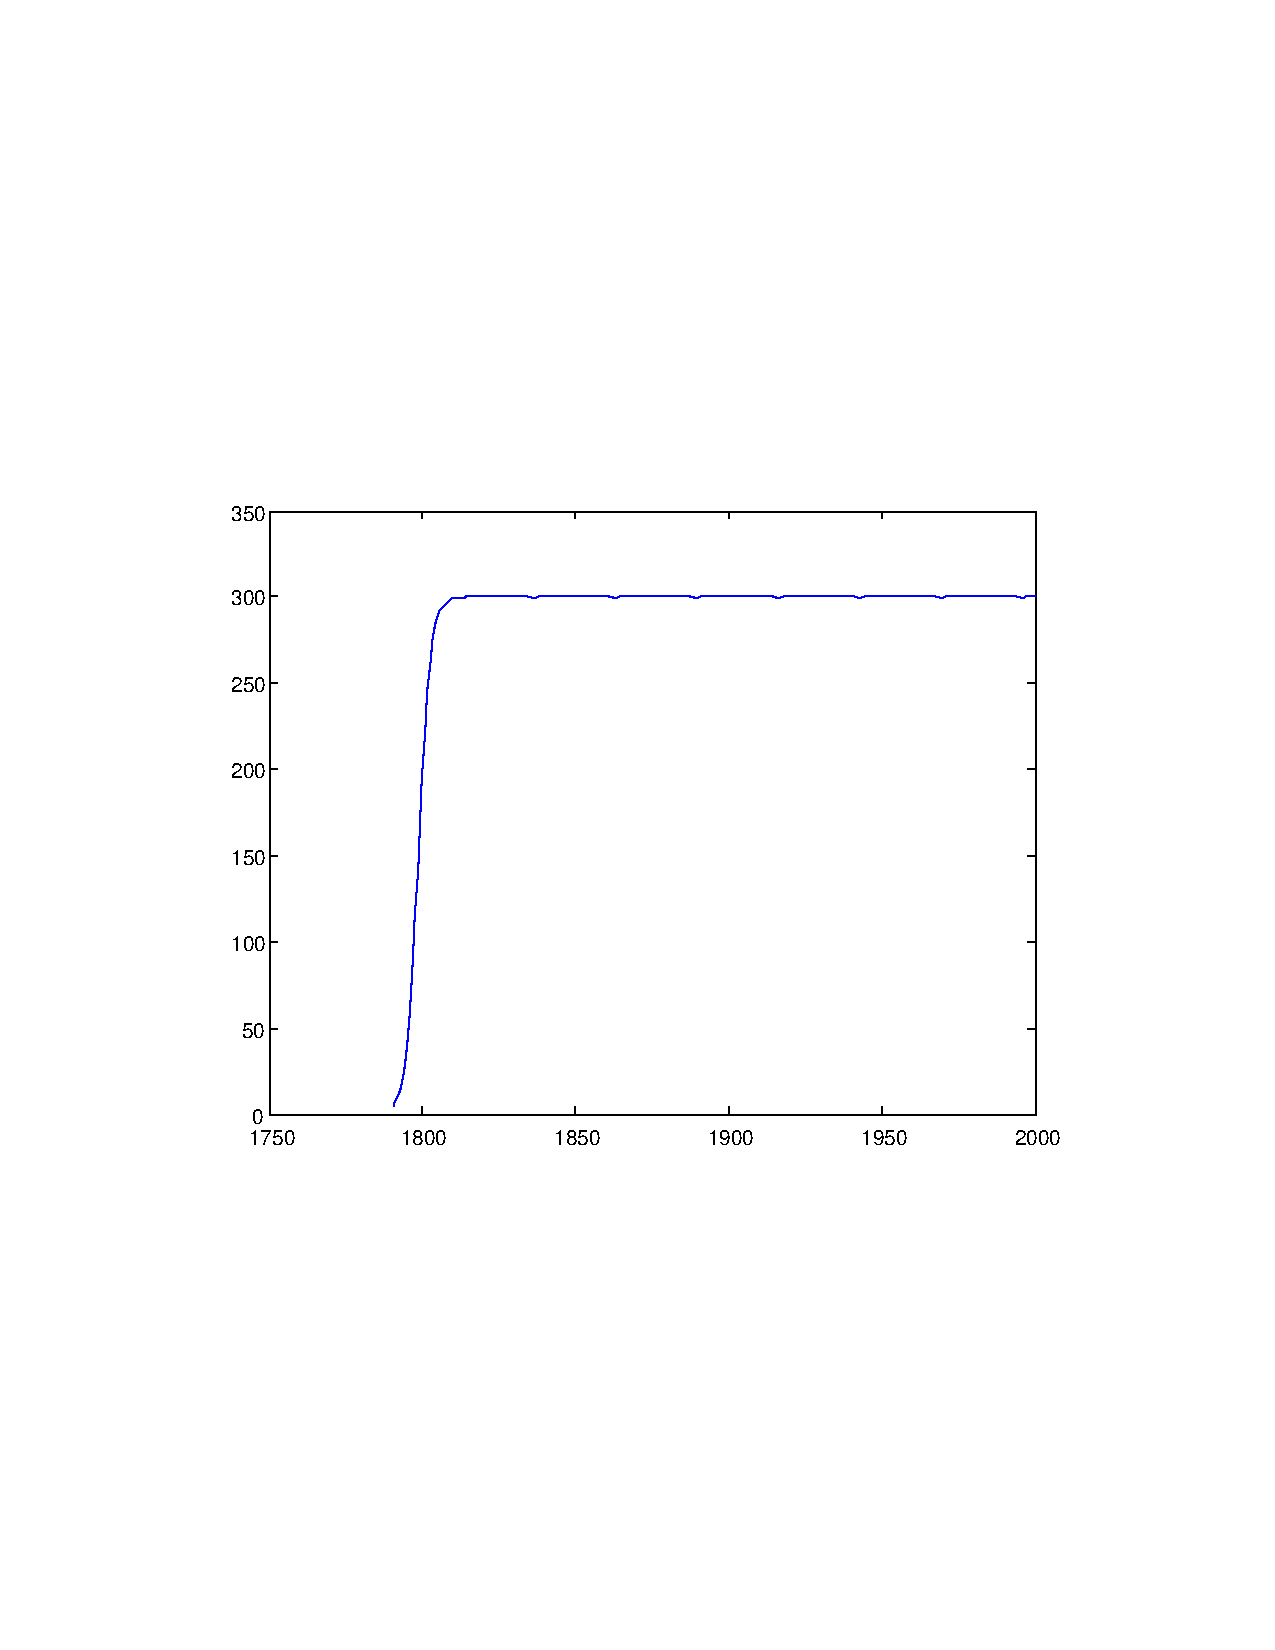
\includegraphics[width=0.7\textwidth]{FIGS/fig_logistic_ode_1}
\end{figure}
}

\frame[containsverbatim]{\frametitle{Tightening the $x$-axis}
\begin{verbatim}
plot(t,N)
xlim([t(1) t(end)])
\end{verbatim}
gives
\begin{figure}[htbp]
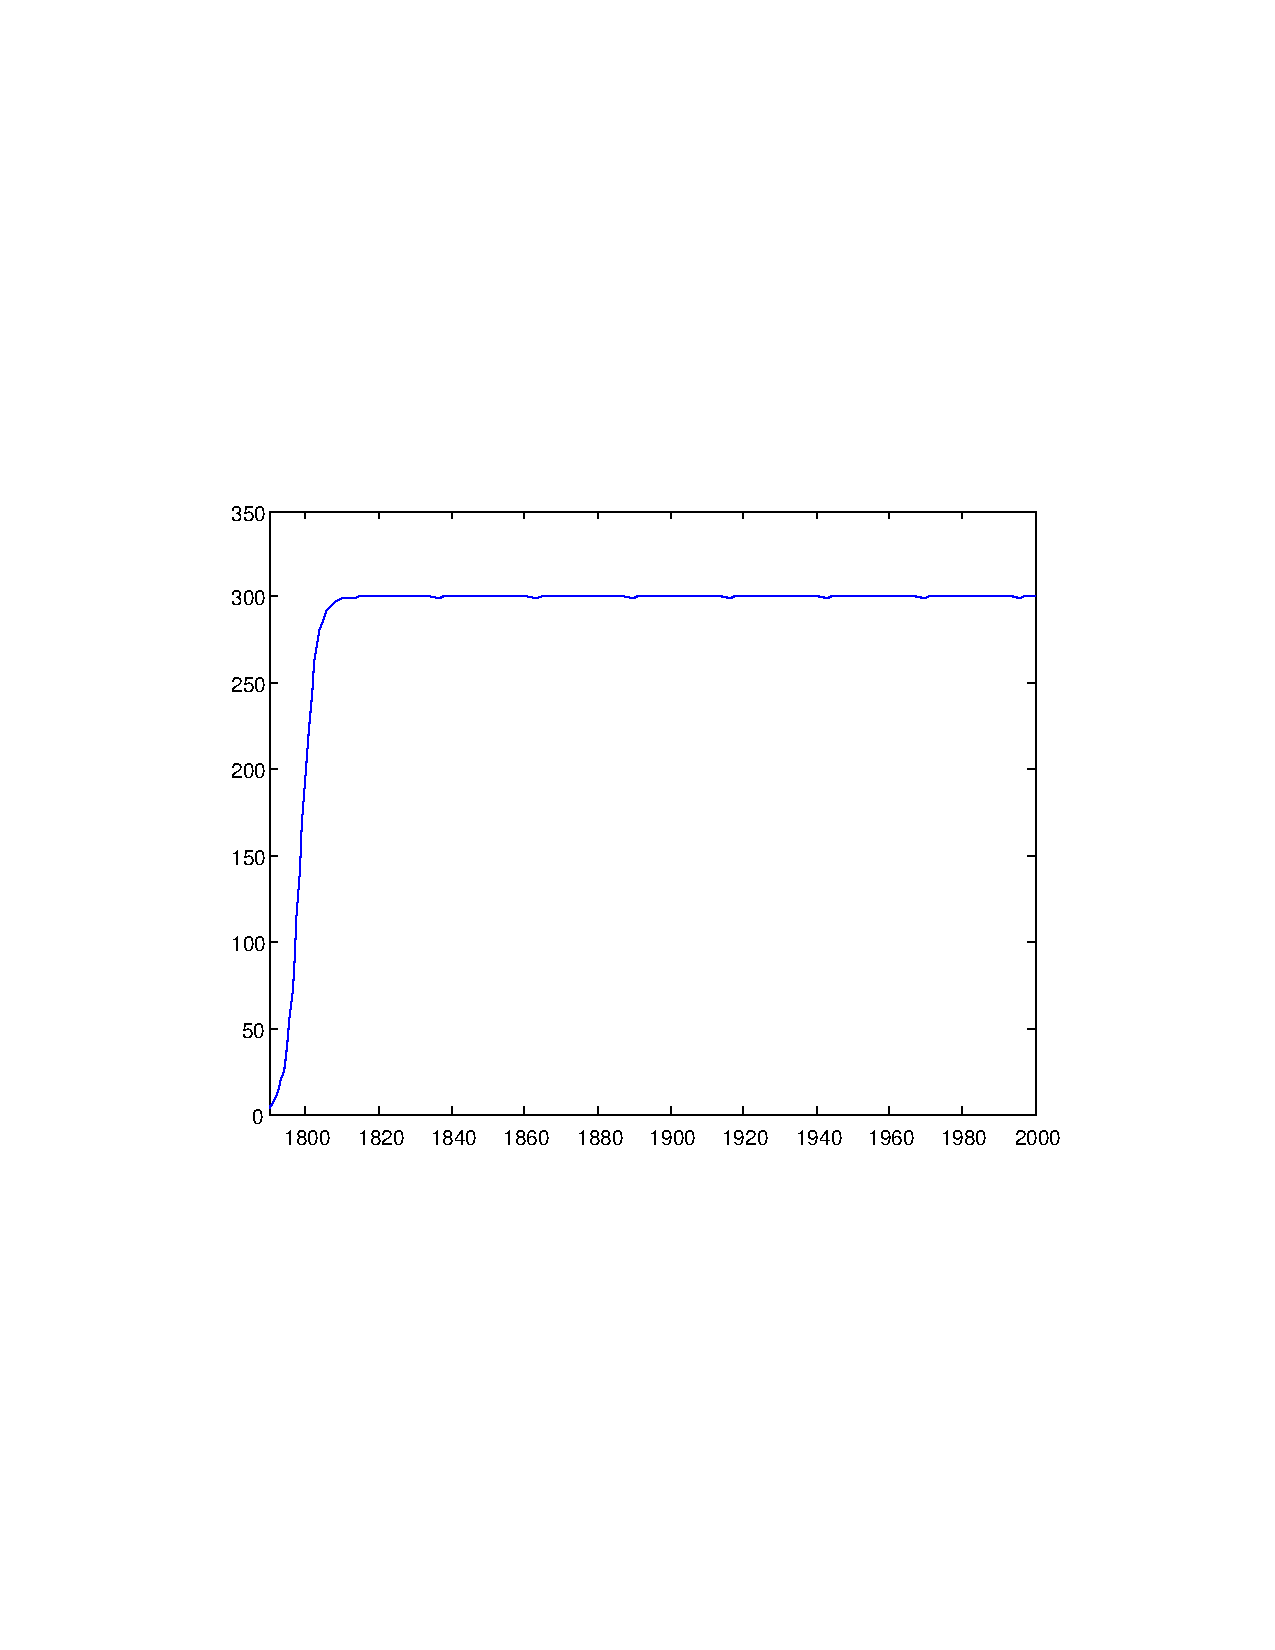
\includegraphics[width=0.7\textwidth]{FIGS/fig_logistic_ode_2}
\end{figure}
}

\frame[containsverbatim]{\frametitle{Using Octave}
The syntax in Octave is almost identical to the matlab syntax. In fact, if you use the additional programs in the {\tt forge} repository, a function {\tt ode45} is defined
\vskip0.5cm
However, the functions (in octave) do not implement the use of a parameter by default, so a work-around must be used
\vskip0.5cm
Update: as of V3.0 and using ode45, parameters can be passed and the matlab code given before works, with the following little modification:
\begin{verbatim}
opt=odeset('InitialStep',0.05,'MaxStep',1);
[t,N]=ode45(@rhs_logistic,tspan,IC,opt,p);
\end{verbatim}
which makes sure that the time step does not become too large)
}


\frame[containsverbatim]{\frametitle{Using scilab}
The syntax in scilab differs a little from matlab, so beware.
\begin{verbatim}
function ydot=f(t,y);
ydot=y^2-y*sin(t)+cos(t);
endfunction
\end{verbatim}
}





\end{document}
